\documentclass[a4paper,12pt, final]{article}
\usepackage{graphicx}
\usepackage[]{fancyhdr}
\usepackage[ngerman]{babel}
\usepackage{geometry}
\usepackage{graphicx}
\usepackage[pages=some]{background}
\usepackage{textpos}
\usepackage{tikz}
\usepackage{hyphenat}
\usepackage{pgfplots}
\usepackage{amsmath}
\usepackage{xcolor}
\usepackage{booktabs}
\usepackage{amssymb}
\usepackage{mathtools}
\usepackage{lmodern}
\usepackage{acronym}
\usepackage{titlesec}
\usepackage{chngcntr}
\usepackage{standalone}
\usepackage[nottoc]{tocbibind}
\usepackage{amsthm}
\usepackage{csquotes}
\usepackage{float}
\usepackage{caption}
\usepackage{etoolbox}
\usepackage{longtable}
\usepackage{xpatch,letltxmacro}
\LetLtxMacro{\cminted}{\minted}
\let\endcminted\endminted
\xpretocmd{\cminted}{\RecustomVerbatimEnvironment{Verbatim}{BVerbatim}{}}{}{}
\usepackage{url}
\usepackage[hidelinks, colorlinks=true, urlcolor=blue, citecolor=black, linkcolor=black]{hyperref} 
\usepackage{algorithm}
\usepackage[acronym, nopostdot,nonumberlist,numberedsection]{glossaries}
\usepackage{algpseudocode}
\usepackage[outputdir=../]{minted}
\captionsetup{singlelinecheck=false, justification=centering, font=small}
\usepackage[backend=biber, style=apa, sorting=nty]{biblatex}
\setlength{\bibitemsep}{1em}
\addbibresource{docs/sources.bib}

\renewcommand{\glossarysection}[2][]{}

\counterwithin{figure}{section}

\DeclareLabeldate{
  \field{date}
  \field{year}
  \field{eventdate}
  \field{origdate}
  \literal{o. D.}
}

\def\UrlFont{\ttfamily\color{blue}}
\DeclareFieldFormat{url}{
  -- URL \url{#1}}

\makenoidxglossaries

\newacronym{o. g.}{o. g.}{oben genannt(en)}
\newacronym{bzw.}{bzw.}{beziehungsweise}
\newacronym{eng.}{eng.}{englisch}
\newacronym{S.}{S.}{Seite}
\newacronym{vgl.}{vgl.}{vergleiche}
\newacronym{o. D.}{o. D.}{ohne Datum}
\newacronym{d. h.}{d. h.}{das heißt}
\newacronym{i. d. R.}{i. d. R.}{in der Regel}

\pgfplotsset{compat=1.18}


\addto{\captionsenglish}{%
  \renewcommand*{\contentsname}{Inhalt}
  \renewcommand*{\listfigurename}{Abbildungen}
  \renewcommand*{\listtablename}{Tabellen}
  \renewcommand*{\figurename}{Abb.}
  \renewcommand*{\tablename}{Tab.}
}

\title{Projektarbeit}
\author{Julius Backes | Tom Kurzke}
\date{Dezember 2024}

\geometry{
 a4paper,
 left=3cm,
 right=2cm,
 top=3cm,
 bottom=2cm
 }

% Header and Footer settings 
\pagestyle{fancy}
\fancyhf{}
\fancyhead[RO]{\nouppercase{\leftmark\hfill}}
\fancyfoot[R]{\thepage}
\setlength{\headheight}{14.49998pt}

\fancypagestyle{plain}{
    \fancyhf{}
    \renewcommand{\headrulewidth}{0pt}
    \fancyfoot[R]{\thepage}
}

\titleformat{\section}
  {\normalfont\Large\bfseries} 
  {\thesection} 
  {1em} % Abstand
  {\thispagestyle{plain}}


\begin{document}

\pagestyle{fancy}
\usetikzlibrary {
    arrows.meta,
    graphs,
    graphdrawing,
    matrix,
    ext.node-families,
    ext.positioning-plus,
    ext.paths.ortho
} 
\usegdlibrary {layered}

\backgroundsetup{
scale=1,
color=black,
opacity=1,
angle=0,
contents={%
  
\includegraphics[width=19cm,height=28.5cm]{docs/logos/background.png}
  }%
}

\begin{titlepage}
\BgThispage
\begin{textblock}{1.5}[1,0.5](0,0.5)
	
\includegraphics[width=6.5cm]{docs/logos/logoronzelen.png}\\[3.5cm]
  \end{textblock}
  

  
\bigskip
\bigskip
\begin{center}
{ \large{Oberschule an der Ronzelenstraße\\[0.2cm]
\textit{Mathematik} und \textit{Informatik}}}\\[1cm]

{\large \textbf{Projektarbeit im Rahmen der Qualifikationsphase}}\\[0.6cm]

% Title
\rule{\linewidth}{0.5mm} \\[0.1cm]
{ \huge \bfseries Zeitliche Optimierung der Klausurenplanung an Schulen mithilfe von Graphentheorie — eine Web-App-Entwicklung
 \\[0.1cm] }
\rule{\linewidth}{0.5mm} \\[1.5cm]

% Authors and supervisor
\noindent

{\large  
    2024/2025
  } \\[1cm] 

{\Large  
    Julius Backes | Tom Kurzke
  } \\

\begin{center}
    \documentclass{standalone}

\usepackage{tikz, pgfplots}
\pgfplotsset{compat=1.8}

\begin{document}

\usetikzlibrary{graphs}
\tikz [nodes={draw, circle}]{
  \node[fill=red!30] (x_1) at (0,0) {MAT};
  \node[fill=blue!30] (x_2) at (1.5,-2) {INF};
  \node[fill=green!30] (x_3) at (1.25,1.5) {GES};
  \node[fill=yellow!30] (x_4) at (-2.5,-1.5) {PHY};
  \node[fill=purple!30] (x_5) at (-2,1.5) {ENG};

  \graph {
    (x_1) -- {(x_3), (x_4), (x_5)},
    (x_2) -- {(x_3), (x_4)},
    (x_4) -- (x_5)
  };
}

\end{document}

\end{center}

{\textit{Betreuende \& Prüfende Lehrer:}}\\[0.3cm]
 {Hr. V. Wolff (Mathematik LK) \& Hr. O. Huras (Informatik GK)}




\end{center}


\end{titlepage}

\pagenumbering{roman}

\thispagestyle{plain}
\newpage
\noindent\textbf{Julius Backes \& Tom Kurzke}\\\\
\textbf{Thema}\\
Zeitliche Optimierung der
Klausurenplanung an Schulen
mithilfe von Graphentheorie — eine
Web-App-Entwicklung\\\\\\
\textbf{Leitfrage}\\
Wie lässt sich mithilfe von Graphentheorie und der Entwicklung einer Web-App die Klausurenplanung an Schulen zeitlich optimieren?\\\\\\
\textbf{Stichworte}\\
Graphentheorie, Graph Coloring, DSatur, Klausurenplanung\\\\
\textbf{Kurzzusammenfassung}\\
Diese Arbeit behandelt die automatisierte Planung von Prüfungsterminen für Schülerinnen und Schüler mithilfe eines graphentheoretischen Ansatzes. Durch den angepassten Dsatur-Algorithmus wird versucht, eine möglichst optimale Verteilung der Klausuren über mehrere Wochen zu erreichen, wobei schulische und organisatorische Anforderungen berücksichtigt werden.


\newpage

\tableofcontents

\newpage

\listoffigures
\vspace{1cm}
\noindent \textit{Hinweis: Alle Abbildungen wurden eigenständig mit dem \LaTeX-Paket TikZ oder Excel erstellt. Eine Quellenangabe ist daher nicht erforderlich.}
\input{docs/chapters/07_abkürzungen}
\newpage
\section{Einleitung}
Die Erstellung eines ausbalancierten Klausurenplans stellt eine große Herausforderung dar, da verschiedene Anforderungen berücksichtigt werden müssen. In diesem Kapitel gehen wir auf die Problemstellung, die Motivation für die Arbeit und die Ziele des Projektes ein.

\subsection{Problemstellung}
Die Planung der Klausuren in der Oberstufe ist aufgrund der Vielzahl an Fächern und Kursen äußerst komplex und zeitaufwendig. Dies führt häufig zu einer unausgewogenen Verteilung der Klausuren. Der Klausurenplan muss dabei bestimmten Regeln folgen: So darf ein Schüler nicht mehr als eine Klausur pro Tag und maximal drei Klausuren pro Woche schreiben. Idealerweise sollte ein Schüler sogar weniger als drei Klausuren pro Woche schreiben.

\subsection{Motivation}
In den letzten Jahren haben wir selbst während unserer Zeit in der Oberstufe der Oberschule an der Ronzelenstraße erfahren, wie schwierig es ist, einen ausgewogenen Klausurenplan zu erstellen. Die Erstellung ist für die zuständigen Lehrkräfte mit einem erheblichem Zeitaufwand verbunden. Häufig wurde der Klausurenplan erst eine Woche vor Beginn der Klausurenphase veröffentlicht. Für uns Schüler war dies sehr frustrierend, da dies bedeutete, dass man erst spät mit Vorbereitung auf die Klausuren beginnen konnte.

\subsection{Ziel der Arbeit}
Um in Zukunft die o. g. Probleme zu vermeiden und den Prozess der Klausurplanung zu optimieren, entwickeln wir im Rahmen dieser Projektarbeit eine Web-App, die folgende Anforderungen erfüllt: Aus einer Excel-Datei, die die Kurse und Schüler beinhaltet und vom Nutzer hochgeladen wird, soll ein Klausurenplan für die eingegebenen Kurse erstellt werden. Zudem sollen die folgenden Anforderungen an den Klausurenplan sichergestellt werden:

\begin{enumerate}
    \item Kurse, in denen zwei Klausuren pro Halbjahr vorgesehen sind, sollen entsprechend umgesetzt werden.
    \item Ein Schüler darf maximal eine Klausur pro Tag schreiben und keine Klausuren zur gleichen Zeit haben.
    \item Ein Schüler darf maximal drei Klausuren pro Woche schreiben.
\end{enumerate}

\pagenumbering{arabic}
\newpage
\section{Grundlagen der Graphentheorie}
Im vorliegenden Kapitel werden grundlegende Konzepte der Graphentheorie eingeführt. 
Diese sind essenziell, um ein tiefes Verständnis von der Funktionsweise der finalen Anwendung zu entwickeln.\\\\
Die Graphentheorie stellt einen Teilbereich der Mathematik dar, der sich mit der Untersuchung von Graphen befasst. 
Die Graphentheorie stellt eine wesentliche Grundlage zur Erstellung und Analyse mathematischer Modelle dar und findet darüber hinaus Anwendung bei der Lösung von Optimierungsproblemen.
\subsection{Grundbegriffe}
Ein Graph aus der Graphentheorie unterscheidet sich signifikant von einem "typischen" Graphen, wie man aus der Schulmathematik und aus der Analysis kennt.\\\\
Ein graphentheoretischer Graph $G$ besteht aus einer Menge von Knoten (engl. vertices), die durch Kanten (engl. edges) miteinander verbunden sein können. 
Diese Knoten können gar nicht oder mehrfach mit anderen Knoten verbunden sein. 
Wenn ein Knoten mit sich selbst verbunden ist, spricht man von einer Schleife. \\\\
Ein Graph $G$ wird formal als ein Paar $G = (V(G), E(G))$ definiert, wobei \(V(G)\) die Menge der Knoten darstellt, beispielsweise \(\{1, 8, 7\}\) oder \(\{A, B, C\}\), und \(E_G\) die Menge der Kanten ist, also Verbindungen zwischen jeweils zwei Knoten.
Für die Kantenmenge \(E(G)\) gilt: 
\begin{equation*}
    E(G) = \{\{v_x, v_y\} \colon \; v_x, v_y \in V(G) \wedge v_x \neq v_y\}
\end{equation*}
Die Einschränkung $v_x \neq v_y$ ist optional.
Dadurch wird festgelegt das es keine Schleifen in dem Graphen geben darf \parencite[2]{Diestel2017-bj}.
In dieser Arbeit werden Schleifen nicht genutzt. Zwei Knoten $a$ und $b$ nennt man benachbart bzw. adjazent (engl. adjacent) wenn $\{a,b\} \in E(G)$ gilt. 
Um die Darstellung zu vereinfachen, definieren wir $E(G) = \{\{A,B\},\{A,C\}\}$ als $E_G = \{AB, AC\}$ \parencite[3]{Diestel2017-bj}.
\begin{figure}[H]
    \centering
    \documentclass{standalone}

\usepackage{tikz, pgfplots}
\pgfplotsset{compat=1.8}

\begin{document}

\usetikzlibrary {graphs}
\tikz [nodes={draw, circle, fill=blue!70}, text=white]{
  \node (a) at (0,0) {$A$};
  \node (b) at (1,1) {$B$};
  \node (c) at (1,-1) {$C$};
  \node (d) at (2,0) {$D$};

  \graph { (a) -- {(b), (c)} -!- (d) };
}

\end{document}
    \caption[caption]{Ein einfacher ungerichteter Graph $G$ \\ mit $V(G)=\{A,B,C,D\}$ und $E(G)=\{{AB, AC}\}$ }
    \label{g1}
\end{figure}
Die Anzahl der Kanten an einem Knoten $v$ wird durch den Grad des Knotens beschrieben. 
Ein Knoten, der mit $n$-vielen Knoten verbunden ist, hat den Grad $n$. Es gilt
$$\deg(v) = |E(v)|$$
Die Knoten werden in schwach verzweigte und stark verzweigte Knoten unterteilt. 
Ein Knoten mit z.B. acht verbundenen Knoten ist stärker verzweigt als ein Knoten mit zwei verbundenen Knoten \parencite[5]{Diestel2017-bj}.\\\\
Graphen lassen sich in zwei Arten unterscheiden: gerichtete Graphen und ungerichtete Graphen. Ein ungerichteter Graph zeichnet sich dadurch aus, dass die Kanten zwischen den Knoten keine Richtung aufweisen (vgl. Abb. 1). Im Unterschied dazu besteht die Kantemenge $E(G)$ eines gerichteten Graphen aus einer Menge von geordneten Paaren anstelle einer Menge von Mengen mit Knoten. Sie wird mit
\begin{equation*}
    E(G) = \{(v_x, v_y) \colon v_x,v_y \in V(G) \wedge v_x \neq v_y\}
\end{equation*}
definiert. Die Kanten eines gerichteten Graphen werden i. d. R. mit einem Pfeil dargestellt \parencite[30]{Diestel2017-bj}.
\begin{figure}[H]
    \centering
    \documentclass{standalone}

\usepackage{tikz, pgfplots}
\pgfplotsset{compat=1.8}

\begin{document}

\usetikzlibrary {graphs}
\tikz [nodes={draw, circle, fill=green!40}]{
  \node (a) at (0,0) {$A$};
  \node (b) at (2,0.5) {$B$};
  \node (c) at (1,-1) {$C$};
  \node (d) at (2,-1) {$D$};

  \graph { (c) -> {(a), (b), (d)}, (d) -> (b) };
}

\end{document}
    \caption[caption]{Ein einfacher gerichteter Graph\\ mit $V(G)=\{A,B,C,D\}$ und $E(G)=\{CA,CB,CD,DB\}$}
\end{figure}
\noindent Sei $N_G(v)$ die Menge aller adjazenten Knoten eines Knoten $v$ in einem Graphen $G$, auch Nachbarn (eng. neighbours) von $v$ genannt. \parencite[5]{Diestel2017-bj}
\begin{equation*}
    N_G(v) \subseteq V(G)
\end{equation*}
\begin{equation*}
    N_G(v)=\{w \in V(G) \colon \{v,w\} \subseteq E(G)  \}
\end{equation*}

\subsection{Graphenfärbung}
Die Knotenfärbung, auch als Graph Coloring bezeichnet, stellt eine Methode zur Färbung von Knoten in einem Graphen $G$ dar. 
Es wird demnach gefordert, dass keine zwei adjazenten Knoten die gleiche Farbe aufweisen.
Die Farben werden i. d. R. als Buchstaben oder Zahlen dargestellt, wobei sie Gruppen oder Zuständen zugeordnet werden.
Das Ziel der Färbung besteht in der Bestimmung der kleinstmöglichen Anzahl an Farben.
Diese Anzahl wird als chromatische Zahl des Graphen bezeichnet.\\\\
Des Weiteren findet die Färbung Anwendung in der Stundenplanerstellung sowie der Färbung von Karten, beispielsweise dem sogenannten Vier-Farben-Satz.
Ein weiteres Anwendungsgebiet stellt die Klausurenplanerstellung dar, wie sie auch in dieser Arbeit erfolgt.\\\\
\newpage
\noindent Mathematisch wird das Graph Coloring als Abbildung $c$ von der Menge $V(G)$ als Knoten auf eine Menge $C(G)$ als Farben für einen Graphen $G$ definiert \parencite[121]{Diestel2017-bj}.
\begin{equation*}
c(v): V(G) \rightarrow C(G)
\end{equation*}
\begin{equation}
\forall \{v_x,v_y\} \in E(G) \colon \; c(v_x) \overset{!}{\neq} c(v_y)
\end{equation}
Mit (1) wird gewährleistet, das zwei adjazente Knoten nicht mit derselben Farbe gefärbt werden.
\vspace{-2.25cm}
\begin{figure}[H]
    \centering
    \documentclass{standalone}
\standaloneconfig{border={-2cm -1.2cm 0 -1.9cm}}

\usepackage{tikz, pgfplots}
\usepackage{amsmath}

\pgfplotsset{compat=1.8}

\begin{document}

\usetikzlibrary {graphs}
\tikz [nodes={draw, circle}, text=white]{
  \node[fill=blue!70] (a) at (-1,2) {$A$};
  \node[fill=red!70] (b) at (1,1) {$B$};
  \node[fill=blue!70] (c) at (2,2) {$C$};
  \node[fill=yellow!70, text=black] (d) at (3,1) {$D$};
  \node[fill=red!70] (e) at (2,-0.5) {$E$};
  \node[fill=yellow!70, text=black] (f) at (-1,0) {$F$};

  \graph { (a) -- {(b) -- {(c), (f)}, (f) -- (e) -- {(d) -- (c), (c)}} };

  \node[anchor=north east, text=black, draw=none] at (current bounding box.north east) [xshift=8cm, yshift=1cm] {
  \footnotesize
    $\begin{aligned}
        V(G)    & = \{A,B,C,D,E,F\}\\
        E(G)    & = \{AB,BC,CD,CE,DE,EF,FA,FB\}\\
        C       & = \{\tikz\draw[fill=blue!70] (0,0) circle (.5ex); , \tikz\draw[fill=red!70] (0,0) circle (.5ex); , \tikz\draw[fill=yellow!70] (0,0) circle (.5ex);\}
    \end{aligned}$
        
  };
}

\end{document}
    \vspace{-2cm}
    \caption{Gefärbter Graph $G$}
\end{figure}
\noindent Ein wichtiges Konzept in der Graphenfärbung ist der \textbf{Sättigungsgrad} (eng. degree of saturation). 
Für einen gegebenen Knoten $v$ beschreibt der Sättigungsgrad $\text{sat}(v)$ die Anzahl der verschiedenen Farben, die in der Menge der Nachbarn vorkommen. Formal gilt: 
\parencite[39]{lewis2021guide}
\begin{equation*}
    \text{sat}(v)=|\{C_G(w)\colon w \in N_G(v) \; \wedge \; w \notin U(G)\}|
\end{equation*}
wobei $C_G(w)$ die Farbe des Knotens $w$ angibt und $U(G)$ die Menge der ungefärbten Knoten. Für $U(G)$ gilt:
\begin{equation*}
    U(G)\coloneqq \{v \in V(G) \colon \;C_G(v) = \varnothing\}
\end{equation*}
Die Funktionen zur Bestimmung des maximalen Sättigungsgrads und des maximalen Knotengrads können wie folgt definiert werden:
\begin{align*}
    \max \text{sat}(v) &= \max(\{\text{sat}(v)\colon \; v \in V(G) \setminus U(G)\})\\
    \max \deg(v) &= \max(\{\deg(v) \colon \; v \in V(G)\})
\end{align*}
TEST2322sasdssasdasdasadas
\newpage
\section{Klausurenplanung als Optimierungsproblem}
EINLEITUNG
\subsection{Modellierung}
Die Klausurenplanung kann effektiv als Graphenproblem modelliert werden, indem die Klausuren und ihre zeitlichen Abhängigkeiten in einem Konfliktgraphen dargestellt werden. In diesem Graphen repräsentiert jeder Knoten eine Klausur $k \in K$, während Kanten zwischen den Knoten Konflikte symbolisieren, die verhindern, dass zwei Klausuren gleichzeitig stattfinden können. Solche Konflikte entstehen beispielsweise, wenn Schüler oder Lehrkräfte an mehreren Klausuren beteiligt sind, da sie nicht gleichzeitig an mehreren Prüfungen teilnehmen können.\\\\
Ein Beispiel veranschaulicht diese Modellierung: Gegeben sei eine Menge von Prüfungen $K(G) = \{A,B,C,D,E\} $, deren Teilnehmer sich überschneiden können. Falls Schüler 1 sowohl an Klausur $A$ als auch an Klausur $B$ teilnimmt, wird eine Kante zwischen den Knoten A und B gezogen. Ebenso entsteht eine Kante zwischen $A$ und $D$, wenn Schüler 2 und Schüler 4 an beiden Klausuren beteiligt sind.
Der resultierende Graph veranschaulicht übersichtlich, welche Klausuren nicht gleichzeitig stattfinden dürfen. Diese Konflikte dienen als Grundlage, um die Klausuren zeitlich so zu planen, dass Überschneidungen vermieden und eine optimale Terminierung gewährleistet werden kann.\\\\
!!ABB.!!\\\\
Das Problem kann mithilfe der Graphenfärbung gelöst werden. Jede Farbe $ c \in C(G)$ repräsentiert ein Datum, und die Aufgabe besteht darin, die Knoten so zu färben, dass keine zwei miteinander verbundenen Knoten dieselbe Farbe erhalten. \\\\
Ziel ist es, die Gesamtzahl der verwendeten Farben zu minimieren, da dies einer Optimierung des Klausurenplans entspricht. Je weniger Farben erforderlich sind, desto kompakter und übersichtlicher wird der Zeitplan, was den organisatorischen Aufwand reduziert.\\\\
Die minimale Anzahl an Farben in einem solchen Konfliktgraphen gibt schließlich an, wie viele Zeitfenster/Tage mindestens benötigt werden, um alle Konflikte zu vermeiden. Dieses Modell bietet eine präzise Grundlage für die Erstellung eines effizienten und konfliktfreien Klausurenplans.\\\\
Wir definieren die Menge der Farben $C(G)$ als die Menge aller möglichen Daten, an denen eine Klausur stattfinden kann. Diese umfasst alle Daten innerhalb eines zuvor festgelegten Zeitraums, ausgenommen Wochenenden, Feiertage und Ferien.\\
Die Menge $WD = \{0, \dots, 4\}$ repräsentiert die Wochentag-Indizes. Wir definieren eine Abbildung 
$$ w_{C(G)} \colon C(G) \rightarrow WD, $$
die jedem Datum einen Wochentag zuweist.\\
Weiterhin definieren wir die Menge $ D = \mathcal{P}(WD) \setminus \varnothing$, also die Potenzmenge von $WD$ ohne die leere Menge. Diese enthält alle möglichen Kombinationen von Wochentag-Indizes. Zusätzlich definieren wir eine Abbildung 
$$ w_{K(G)} \colon K(G) \rightarrow D, $$
die jedem Knoten $v \in K(G)$ eine Teilmenge von $WD$ zuordnet.\\
Die möglichen Farben eines Knotens $v$ definieren wir schließlich als
$$
C(v)= \{ c \colon \; c \in C(G) \, \setminus \, C(N_G(v)) \; \wedge \; w_{C(G)}(c) \in w_{K(G)}(v)\}
$$
wobei $N_G(v)$ die Menge der Nachbarn von $v$ im Graphen $G$ bezeichnet. 

\subsection{Zielsetzungen}
\newpage
\section{Entwicklung der Web-Applikation}
Die Entwicklung der Webanwendung verfolgt das Ziel, einen effizienten und automatisierten Prozess für die Klausurenplanung in der Oberstufe zu schaffen. In diesem Kapitel werden die Anforderungen definiert und die technische Umsetzung beschrieben.
\subsection{Anforderungen und Spezifikationen}
Für eine strukturierte Umsetzung müssen die funktionalen und nicht-funktionalen Anforderungen an die Anwendung definiert werden. Schlussendlich soll im Rahmen der technischen Möglichkeiten eine übersichtliche und benutzerfreundliche Oberfläche geschaffen werden. Eine frühzeitige Differenzierung der Anforderungen erleichtert im allgemeinen die spätere Umsetzung und strukturierte Evaluation.
\subsubsection{Funktionale Anforderungen}
Funktionale Anforderungen definieren, welche konkreten Funktionen und Aufgaben eine Anwendung erfüllen soll. Sie beschreiben, welche Leistungen das System erbringen muss, um die gewünschten Ziele zu erreichen \parencite{anforderungen}. Im Folgenden werden wir die funktionalen Anforderungen in Kernfunktionen und Benutzerfunktionen unterteilen.\\\\
\textbf{Kernfunktionen}
\begin{itemize}
    \item Die Web-Applikation soll automatisiert einen Klausurenplan im Excel-Format erstellen, basierend auf den vom Benutzer übermittelten Daten.

    \item Der Klausurenplan sollte die Anzahl der verschiedenen Klausurtage minimieren und dabei die folgenden Regeln berücksichtigen:
    \begin{itemize}
        \item Maximal drei Klausuren pro Schüler pro Woche.
        \item Maximal eine Klausur pro Schüler und Tag.
        \item Keine Klausuren an Feiertagen oder während der Schulferien.
    \end{itemize}

    \item Die Web-Anwendung sollte den Klausurenplan und die dazugehörigen Graphen visualisieren können.
\end{itemize}
\textbf{Benutzerfunktionen}
\begin{itemize}
    \item Dem User soll die Möglichkeit gegeben werden, folgende Daten hochzuladen und auszuwählen:
    
    \begin{itemize}
        \item Der User soll eine Kursliste im Excel-Format herunterladen können. Diese soll alle Kurse mit ihren Schüler enthalten. Daraus soll für jeden Kurs eine Liste erstellt werden, welche Kurse nicht gleichzeitig mit dem Kurs stattfinden können.
        
        \item Der User sollte Kurse auswählen können, die zweimal pro Halbjahr eine Klausur schreiben.
        
        \item Der User sollte, jedem Kurs mindestens einen oder mehrere mögliche Prüfungstage (Wochentage) zuzuweisen können.
        
        \item Der User sollte einen Zeitraum festlegen können, in dem alle Klausuren stattfinden sollen. Diesen Zeitraum nennen wir Klausurenphase.
    \end{itemize}
    
    \item Alle o. g. Daten sollten von dem Benutzer geändert werden können. 
    
    \item Es sollte möglich sein, die Klausurenpläne in verschiedenen Projekten zu strukturieren, um eine bessere Übersicht zu gewährleisten. 
    \item Die Projekte sollten nur für den Ersteller zugänglich sein.
\end{itemize}
\subsubsection{Nicht-funktionale Anforderungen}
Nichtfunktionale Anforderungen umfassen alle Anforderungen, die nicht die Funktion, sondern die Qualität des Endprodukts bestimmen \parencite{anforderungen}.
\begin{itemize}
    \item Die Web-App soll performant sein und auch bei vielen Kursen und Schülern schnell einen Klausurenplan erstellen.
    \item Das Design der Webanwendung sollte modern, minimalistisch und konsistent sein.
    \item Auf die Benutzerfreundlichkeit ist zu achten. Funktionen sollten nicht versteckt, sondern leicht verständlich und intuitiv  sein.
    \item Der Quellcode der Webanwendung sollte sinnvoll strukturiert, fehlerfrei und wiederverwendbar sein.
    \item Moderne Web-Technologien sollen eingesetzt werden, um eine robuste und zukunftssichere Entwicklung zu gewährleisten.
\end{itemize}
\subsection{Systemarchitektur}
Die Systemarchitektur umfasst alle wichtigen Technologien und Werkzeuge, die zur Implementierung der Webanwendung verwendet werden. Sie beschreibt die grundlegende Struktur der Anwendung, einschließlich der Trennung zwischen Frontend und Backend und deren Interaktion. Das Frontend ist für die Benutzeroberfläche zuständig, während das Backend die Datenverarbeitung und Logik übernimmt \parencite{mccartney-2024}. Die Kommunikation zwischen beiden Bereichen erfolgt über standardisierte Schnittstellen. So genannte Application Programming Interfaces (APIs) \parencite{gazarov-2019}. Ziel der Architektur ist es, eine skalierbare, wartbare und performante Anwendung zu schaffen, die effizient weiterentwickelt werden kann.
\subsubsection{Frontend-Design}
Das Frontend-Design befasst sich mit der Benutzeroberfläche. Welche Werkzeuge werden verwendet, um dem Benutzer welche Funktionen auf welche Weise anzuzeigen? \parencite{mccartney-2024}\\\\
Das Grundgerüst einer Webseite wird mithilfe der Hypertext Markup Language (HTML) erstellt. Elemente können durch Cascading Style Sheets (CSS) mit Attributen wie Farbe, Textgröße und Ähnlichem versehen werden. Die Logik für Animationen sowie die Interaktion mit der Webseite wird über die Programmiersprache JavaScript (JS) gesteuert \parencite{mdn-getting-started-web}. Obwohl der Name es vermuten lassen könnte, besteht kein Zusammenhang zwischen JavaScript und der Programmiersprache Java \parencite{geeksforgeeks-2024}.\\\\
JavaScript wird in der Regel direkt im Browser ausgeführt. Es handelt sich um eine dynamisch typisierte Sprache, d.h. Variablen und Funktionen können ähnlich wie in Python ohne explizite Typenangaben definiert werden \parencite{mdn-javascript}. Dies kann allerdings zu einfachen Fehlern führen. Um dem entgegenzuwirken, wird in modernen Webanwendungen häufig TypeScript verwendet. TypeScript ist eine Erweiterung von JavaScript, bei der Typen explizit angegeben werden müssen. Nach der Entwicklung wird TypeScript in reguläres JavaScript kompiliert \parencite{typescript-tutorial-2024}.
\begin{minted}{javascript}
let x = 42;
x = "Hello, World!";
\end{minted}
In JavaScript würde der obige Code keinen Fehler verursachen, da die Variable \texttt{x} keinen festen Typ hat. In TypeScript hingegen würde bereits während der Entwicklung ein Fehler angezeigt werden, da die Variable \texttt{x} ursprünglich als \texttt{number} (Java-Äquivalent: \texttt{int} – ganzzahlige Zahl) deklariert wurde und daher nicht mit einem \texttt{string} (Zeichenfolge) überschrieben werden darf \parencite{typescript-tutorial-2024}.\\\\
In der modernen Webentwicklung nutzt man sogenannte Frameworks. Das sind Software-Bibliotheken, die Entwicklern Werkzeuge, Strukturen und vorgefertigte Funktionen bereitstellen, um die Entwicklung von dynamischen Webanwendungen effizienter und einfacher zu gestalten. Sie bieten eine standardisierte Basis für häufig benötigte Aufgaben wie Routing, die Bereitstellung von Webservern und die Nutzung von Reaktivität \parencite{mdn-intro-to-cs-frameworks}.\\\\
Bekannte Beispiele für Web-Frameworks sind React, Django, Angular und Svelte \parencite{mdn-intro-to-cs-frameworks}. Für dieses Projekt wird das open-source-web-framework Svelte verwendet, da es als modernes und robustes Framework bekannt ist. Im Vergleich zu vielen anderen Frameworks, die mit der Zeit zunehmend komplexer wurden, bietet Svelte einen einfachen und direkten Ansatz. Diese Komplexität bei anderen Frameworks entsteht häufig dadurch, dass neue Probleme durch wachsende Anforderungen und zusätzliche Funktionen gelöst werden mussten \parencite{svelte-rethinking}.\\\\
Svelte verfolgt jedoch einen anderen Ansatz, indem es die meisten Aufgaben bereits während der Kompilierung löst. Dadurch wird weniger JavaScript im Browser ausgeführt, was die Performance verbessert und die Entwicklungsarbeit erleichtert. Die einfache Syntax und die starke Fokussierung auf Benutzerfreundlichkeit machen Svelte besonders attraktiv für moderne Webprojekte \parencite{svelte-rethinking}.\\\\
tailwind - shadcn
\newpage
\subsubsection{Backend-Design}
Das Backend umfasst alle Prozesse, die im Hintergrund der Anwendung ablaufen. Es steuert die Logik für Benutzerfunktionen, verarbeitet Datenbankabfragen, regelt die Kommunikation zwischen Diensten und sorgt dafür, dass Funktionen wie Benutzerauthentifizierung reibungslos funktionieren \parencite{nam-le-thanh-web-designer-2023}.\\\\
Das Backend der hier entwickelten Webanwendung soll vor allem zwei Hauptaufgaben erfüllen. Erstens die Authentifizierung: Dazu gehören die Speicherung von Benutzerdaten, die Verschlüsselung von Passwörtern und die Speicherung von sogenannten Authentifizierungstokens, die für die Kommunikation mit dem Backend benötigt werden. Zweitens die Speicherung aller anderen Daten. Alle Kurse, Graphen und alle damit verbundenen Daten müssen gespeichert werden.\\\\
Dazu benötigt man eine Datenbank. In diesem Projekt wird eine SQL-Datenbank (Structured Query Language) verwendet, da es durch die feste Datenstruktur und die einfache Verwaltung von Beziehungen ideale Voraussetzungen für die sichere und einheitliche Speicherung komplexer Daten wie Kurse und Graphen bietet \parencite{aws-sql}.\\\\
Nun muss noch eine Lösung für die andere Hauptaufgabe gefunden werden. Die Antwort heißt Firebase bzw. Supabase. Firebase ist ein Backend-as-a-Service (Baas), das von Google entwickelt wurde. Es ist Cloud-basiert und hat viele wichtige Funktionen wie Datenbank, Authentifizierung und vieles mehr bereits integriert. Supabase ist eine Open-Source-Kopie von Firebase \parencite{wilson-2022}. Unternehmen wie Mozilla, PwC, Johnson \& Johnson und 1Password verwenden Supabase \parencite{sb-companies}.\\\\

sveltekitt?\\\\\\\\
Alle Voraussetzungen sind erfüllt: Die Benutzeroberfläche wird mit TypeScript und dem Framework Svelte entwickelt. Im Backend übernimmt Supabase sowohl die Datenbankverwaltung als auch die Benutzerauthentifizierung und bildet damit eine stabile und skalierbare Grundlage für die Anwendung.
\newpage
\subsection{Implementierung}
EINLEITUNG
\subsubsection{Algorithmische Umsetzung}
In der Anwendung wird ein Dsatur (Degree of Saturation - Grad der Sättigung ) Algorithmus verwendet.

\begin{algorithm}
\caption{Dsatur Algorithmus in Pseudocode}\label{alg:cap}
\begin{algorithmic}
\Require Graph $G = (V(G), E(G))$, Farben $C(G)$\\
\State coloring $\gets$ $f: V(G) \rightarrow \varnothing$\\



\While{$U(G)$ $\neq$ $\varnothing$}

    \State chosenVertex $\gets$ $\arg \max \text{sat($U(G)$)}$\\
    
    \If{(chosenVertex $=$ $\varnothing) \vee (\text{chosenVertex} \in \mathcal{P}(V(G))$}\\
        \State chosenVertex $\gets$ $\arg \max \deg(U(G))$\\
        
        \If{chosenVertex = $\varnothing$}\\
            \State chosenVertex $\gets$ getRandomVertex($U(G)$)\\
        \EndIf\\
    \EndIf\\
    \State lowestColor $\gets$ getLowestAvailableColor(chosenVertex)
    \State coloring.set(chosenVertex, lowestColor)\\
\EndWhile

\end{algorithmic}
\end{algorithm}
\subsubsection{Benutzeroberfläche}
\newpage

\section{Analyse und Evaluation der Optimierung}
In diesem Kapitel werden die Optimierungsergebnisse analysiert und bewertet. Dazu wird zunächst die Qualität der gefundenen Lösung anhand definierter Metriken überprüft. Anschließend erfolgt eine Untersuchung der Effizienz und Komplexität des gewählten Algorithmus, um dessen Leistungsfähigkeit zu beurteilen. Abschließend werden die durchgeführten Tests und deren Ergebnisse vorgestellt, um die Praxistauglichkeit der Lösung zu bewerten und Verbesserungspotentiale aufzuzeigen.
\subsection{Bewertung der Lösungsqualität}
Der Algorithmus terminiert grundsätzlich fair und bietet viel Freiraum bei der Planung. Die Regel, nicht mehr als drei Prüfungen pro Schüler pro Woche vorzusehen, ist jedoch bei einer sehr hohen Anzahl von Kursen schwer einzuhalten und kann in diesen seltenen Fällen überschritten werden.\\\\
In Zukunft könnte versucht werden, einen noch schnelleren und optimaleren Algorithmus als den Dsatur-Algorithmus zu finden. Außerdem könnte versucht werden, durch weitere Optimierungen die Regel von maximal drei Klausuren pro Schüler pro Woche besser einzuhalten.\\\\
Ein Aspekt des DSatur-Algorithmus ist die zufällige Auswahl des ersten Knotens. Dies kann dazu führen, dass die Terminierung der Klausuren bei wiederholten Durchläufen leicht variiert. Dies wirkt sich zwar auf die genaue Anordnung der Termine aus, hat aber keinen negativen Einfluss auf die Einhaltung der Planungsregeln und die Gesamtqualität der Lösung.

\subsection{Effizienz und Komplexität}
Der DSatur-Algorithmus durchläuft in jeder Iteration einen Auswahlprozess, bei dem alle noch nicht eingefärbten Knoten geprüft werden. Dieser Prozess wird fortgesetzt, bis alle Knoten eingefärbt sind. Zudem wird in jeder Iteration die Sättigung jedes Knotens abgefragt, um den nächsten Knoten mit der höchsten Sättigung zu bestimmen. Darüber hinaus wird die bestmögliche verfügbare Farbe ermittelt. Insgesamt ergibt sich daraus eine Laufzeit von $\mathcal{O}(n^2)$, wobei $n = |V(G)|$ die Anzahl der Knoten im Graphen ist. \glqq Schnell\grqq \, sind Algorithmen mit nicht-polynomialer Komplexität wie $\mathcal{O}(n)$ oder $\mathcal{O}(\log(n))$ \parencite{leismann-2023}.
Die Big O Notation ($\mathcal{O}(n^2)$) beschreibt, wie die Laufzeit eines Algorithmus mit der Größe des Inputs wächst, und kategorisiert Algorithmen nach ihrer Effizienz \parencite{leismann-2023}.\\\\
\begin{figure}[h!]
\centering
\begin{tabular}{@{}cc@{}}
\toprule
\textbf{Anzahl der Kurse} & \textbf{Laufzeit (s)} \\ \midrule
10                        & 0.612                 \\
100                       & 3.582                 \\
500                       & 13.399                \\
1000                      & 32.197                \\ \bottomrule
\end{tabular}
\caption[Laufzeiten für verschiedene Kursanzahlen]{Laufzeiten für verschiedene Kursanzahlen (durgeführt auf MacBook Air 2020 M1)}
\label{tab:laufzeiten}
\end{figure}
\subsection{Tests und Ergebnisse}
Die Webanwendung wird im Folgenden anhand eines Beispiels getestet. Dabei werden Kurse basierend auf den 11 Kursen des Profils 23PB1 der Oberschule an der Ronzelenstraße verwendet. Um die Kursnummern eindeutig einem Jahrgang zuzuordnen, wird jedem Kursnamen ein Suffix hinzugefügt, das den entsprechenden Jahrgang angibt. Der Test umfasst 11 Kurse für die Einführungsphase (E-Phase), die Qualifikationsphase 1 (Q1-Phase) und die Qualifikationsphase 2 (Q2-Phase), sodass insgesamt 33 Kurse in der Tabelle dargestellt werden.\\\\
Hinter der Jahrgangsstufe ist, abhängig von der Kursart, ein oder zwei Zahlen angegeben. Diese Zahlen repräsentieren den Wochentag-Index (Montag = 0, Freitag = 4). Jede Spalte enthält Schüler aus den entsprechenden Kursen. Die verwendeten Schülerlisten sind jedoch fiktiv und mit einem Suffix für die Jahrgangsstufe versehen, um jahrgangsübergreifende Konflikte zu vermeiden.\\\\
Die zugehörige Excel-Tabelle mit den Daten finden Sie im Anhang (Abb. \ref{fig:studenList}).\\\\
In der Webanwendung wird zunächst ein neues Projekt erstellt, in dem die erforderliche Datei hochgeladen wird. Das System extrahiert alle relevanten Daten selbstständig aus der Datei. Der Zeitraum für den Klausurenplan wird vom Nutzer festgelegt; beispielhaft wurde hier der Zeitraum vom 16.09.2024 bis zum 15.11.2024 gewählt.\\
Sobald alle relevanten Daten bereitgestellt wurden, generiert die Anwendung den Klausurenplan. Dieser ist ebenfalls im Anhang zu finden (Abb. \ref{fig:klausurenplan}). Zusätzlich ist der Graph, der die Beziehungen zwischen den Kursen visualisiert, ebenfalls im Anhang dargestellt (Abb. \ref{fig:graph1}).\\\\
Die folgenden Eigenschaften des vorliegenden Klausurenplans sind deutlich erkennbar: Jeder Kurs ist korrekt dem entsprechenden Jahrgang zugeordnet. Feiertage und Ferientage wurden dynamisch erkannt und berücksichtigt. Zudem ist ersichtlich, dass die Klausuren ausschließlich an den Tagen terminiert sind, an denen sie tatsächlich stattfinden können. Klausuren, die als 2x/Halbjahr (hier LKs) gekennzeichnet sind, wurden gezielt am Anfang und am Ende des Klausurenplans platziert.\\\\
Weiterhin zeigt der Plan, dass Klausuren \acrshort{i. d. R.} in geeigneten Wochen angesetzt sind. Beispielsweise wurden in Kalenderwoche 43 drei Klausuren terminiert. Ein Blick auf die Schülerlisten zeigt jedoch, dass keine dieser Klausuren in direktem Konflikt zueinander steht, sodass sie optimal innerhalb einer Woche stattfinden können. Der Algorithmus nutzt den gesamten verfügbaren Zeitraum und minimiert dabei effizient die benötigten Zeitslots.
\newpage
\section{Zusammenfassung und Ausblick}
\subsection{Zusammenfassung}
In dieser Arbeit haben wir uns mit dem Problem der zeitlichen Optimierung des Klausurenplans befasst und dafür eine Web-Applikation entwickelt, die helfen soll, dieses Problem zu lösen. Ziel der Arbeit war es, eine Webanwendung zu erstellen, die mithilfe von Graphentheorie arbeitet und in kurzer Zeit unkompliziert konfliktfreie Klausurenpläne erstellt.\\\\
Im theoretischen Teil der Arbeit wurden Grundlagen zum Thema Graphentheorie, insbesondere zur Graphenfärbung, dargestellt. Es wurde erklärt, wie mithilfe dieser Methoden zeitliche Überschneidungen zwischen verschiedenen Klausuren vermieden werden können, sodass keine zwei Klausuren, die im Konflikt stehen, gleichzeitig stattfinden. Das Problem wurde in einem Konfliktgraphen abgebildet und durch Färben des Graphen die kleinste Anzahl an Zeiträumen ermittelt. Es wurden Grundlagen zur Programmierung vermittelt und erläutert, warum die Arbeit zum Bau einer Website von Bedeutung ist. Die eingesetzten Werkzeuge im Front- und Backend-Bereich wurden detailliert beschrieben. Der Kernalgorithmus dieser Arbeit ist Dsatur (Degree of Saturation), da er vergleichsweise einfach zu implementieren ist und liefert gute Ergebnisse bei kurzer Laufzeit, was ihn besonders für Anwendungen mit vielen Klausuren und Schülern geeignet macht.\\\\
Im praktischen Teil wurde die Web-Applikation entwickelt, die mithilfe von Graphentheorie in kurzer Zeit ausgeglichene Klausurenpläne erstellt. Die Anwendung verarbeitet vom Nutzer hochgeladene Excel-Dateien mit Schüler- und Kursdaten und erstellt daraus einen Klausurenplan. Die Applikation berücksichtigt dabei die Begrenzung der Klausuren pro Schüler und mit einer Klausur am Tag. Die Klausurtermine sind über den vom Nutzer gewählten Zeitraum gleichmäßig verteilt, um die Schüler zu entlasten. Bei der Gestaltung der Webanwendung stand die Benutzerfreundlichkeit im Vordergrund. Es wurde übersichtlich und minimalistisch gestaltet, um dem Nutzer ein angenehmes Arbeitserlebnis zu bieten.\\\\
Insgesamt bietet die Arbeit eine gute Grundlage für eine schnelle und konfliktfreie Klausurenplanung. Die entwickelte Web-App vereinfacht den Planungsprozess für Lehrkräfte und ermöglicht es, Klausurenpläne rechtzeitig zu erstellen. Dadurch wird der organisatorische Aufwand reduziert und die Vorbereitung für Schüler und Lehrkräfte erleichtert.
\subsection{Ausblick}
Obwohl die Implementierung unserer Webanwendung zur Klausurenplanung erfolgreich abgeschlossen wurde, gibt es noch einige Bereiche, die in Zukunft erweitert oder verbessert werden können. Sowohl die Funktionalität der Anwendung als auch die Benutzerfreundlichkeit bieten Potential für weitere Optimierungen.\\\\
Der verwendete Algorithmus liefert bereits gute Ergebnisse. Dennoch kann versucht werden, die Performance und die Qualität der Ergebnisse durch weitere sinnvolle Metriken zu verbessern. Ein Ansatz hierfür wäre ein noch schnellerer Algorithmus, der noch bessere Lösungen berechnet. Ebenso könnte versucht werden, sogenannte Cluster in den Graphen zu erkennen. Diese würden dann Profil- bzw. freie LKs und GKs repräsentieren. Darüber könnte man versuchen eine lokale Einfärbung durchzuführen, um noch bessere Einfärbungen zu erhalten.\\\\
Die Webanwendung kann derzeit nur für das Bundesland Bremen genutzt werden, da die eingetragenen Feiertage nicht für alle Bundesländer gelten. Um die Feiertage automatisch zu berücksichtigen, könnte die Anwendung um eine Funktion zur Auswahl der Region erweitert werden. Auf diese Weise könnte der Nutzer Klausurpläne für Schulen in jedem beliebigen Bundesland erstellen.\\\\
Eine zukünftige Version der Web-Applikation sollte die Möglichkeit bieten, dem Kalender eigene unterrichtsfreie Tage hinzuzufügen. So könnte der Nutzer Tage auswählen, an denen keine Prüfungen geschrieben werden dürfen, z.B. bei schulinternen Veranstaltungen wie Schüler-Eltern-Lehrer-Gesprächen oder einem pädagogischen Tag.\\\\
Bisher gibt es keine Möglichkeit, sich bei Fragen zur Bedienung oder bei Fehlern an uns zu wenden. Ein User-Support würde dies ermöglichen. Man füllt ein Kontaktformular aus und gibt an, was das Problem ist oder welche Fragen man hat. Wir könnten dann darauf eingehen und den Nutzern helfen, problemlos mit unserer Webanwendung zu arbeiten.\\\\
Diese Erweiterungen würden die Anwendung noch leistungsfähiger, flexibler und benutzerfreundlicher machen und dazu beitragen, den Prozess der Prüfungsplanung weiter zu optimieren.
\newpage
\setcounter{section}{7} % weg vor Prod
\section{Literaturverzeichnis}
\printbibliography
\newpage
\appendix
\section{Anhang}
\subsection{Schülerliste \& Graph}
\subsubsection*{Schülerliste}
\begin{figure}[H]
    \centering
    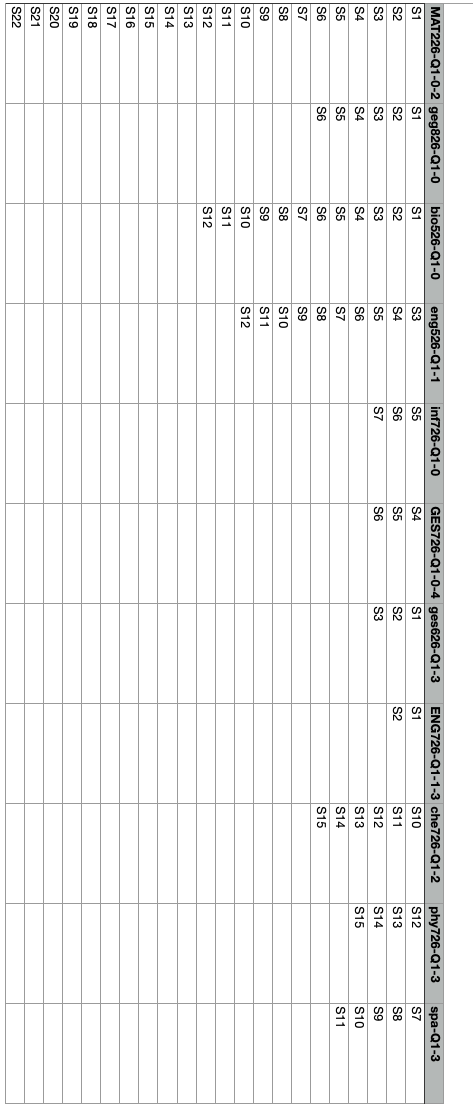
\includegraphics[width=0.5\linewidth]{docs/graphics/StudentList1.png}
    \caption{Schülerliste in Excel-Tabelle (anonymisierte Daten)}
    \label{fig:studenList}
\end{figure}
\begin{figure}[H]
    \centering
    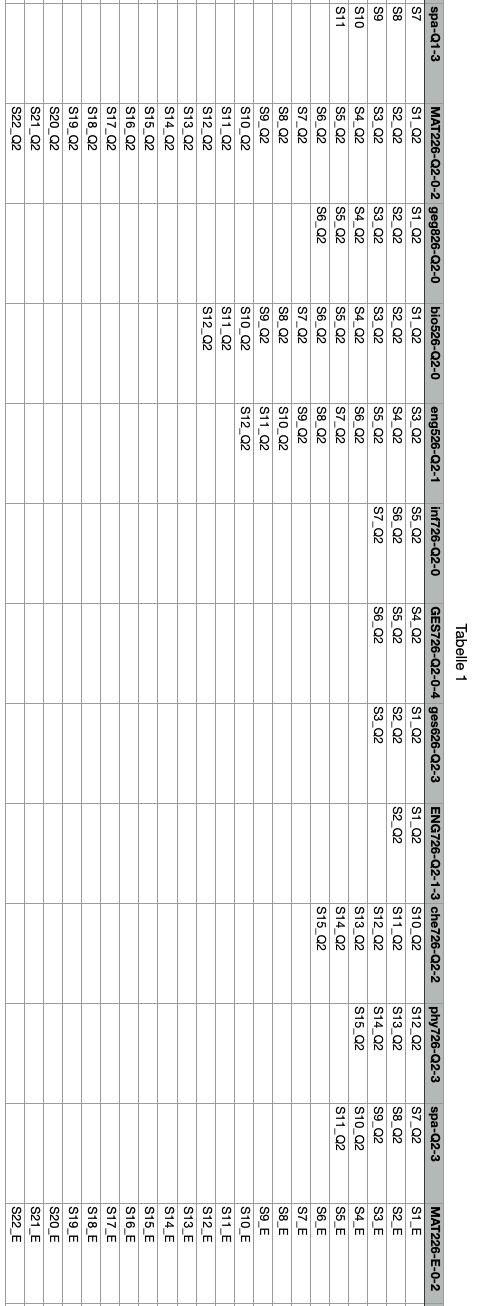
\includegraphics[width=0.6\linewidth]{docs/graphics/StudentList2.png}
\end{figure}
\begin{figure}[H]
    \centering
    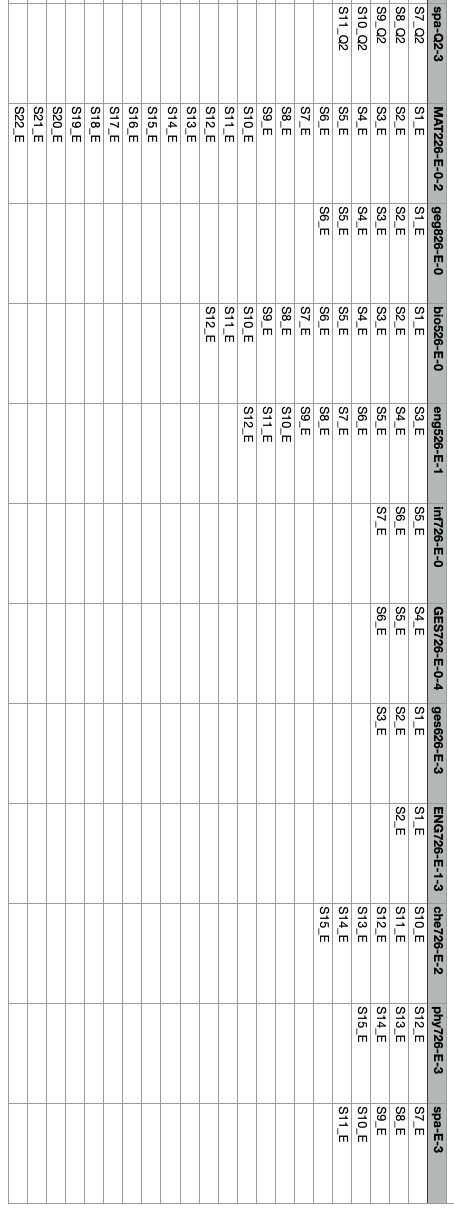
\includegraphics[width=0.6\linewidth]{docs/graphics/StudentList3.png}
\end{figure}

\newpage
\subsubsection*{Graph}
\begin{figure}[H]
    \centering
    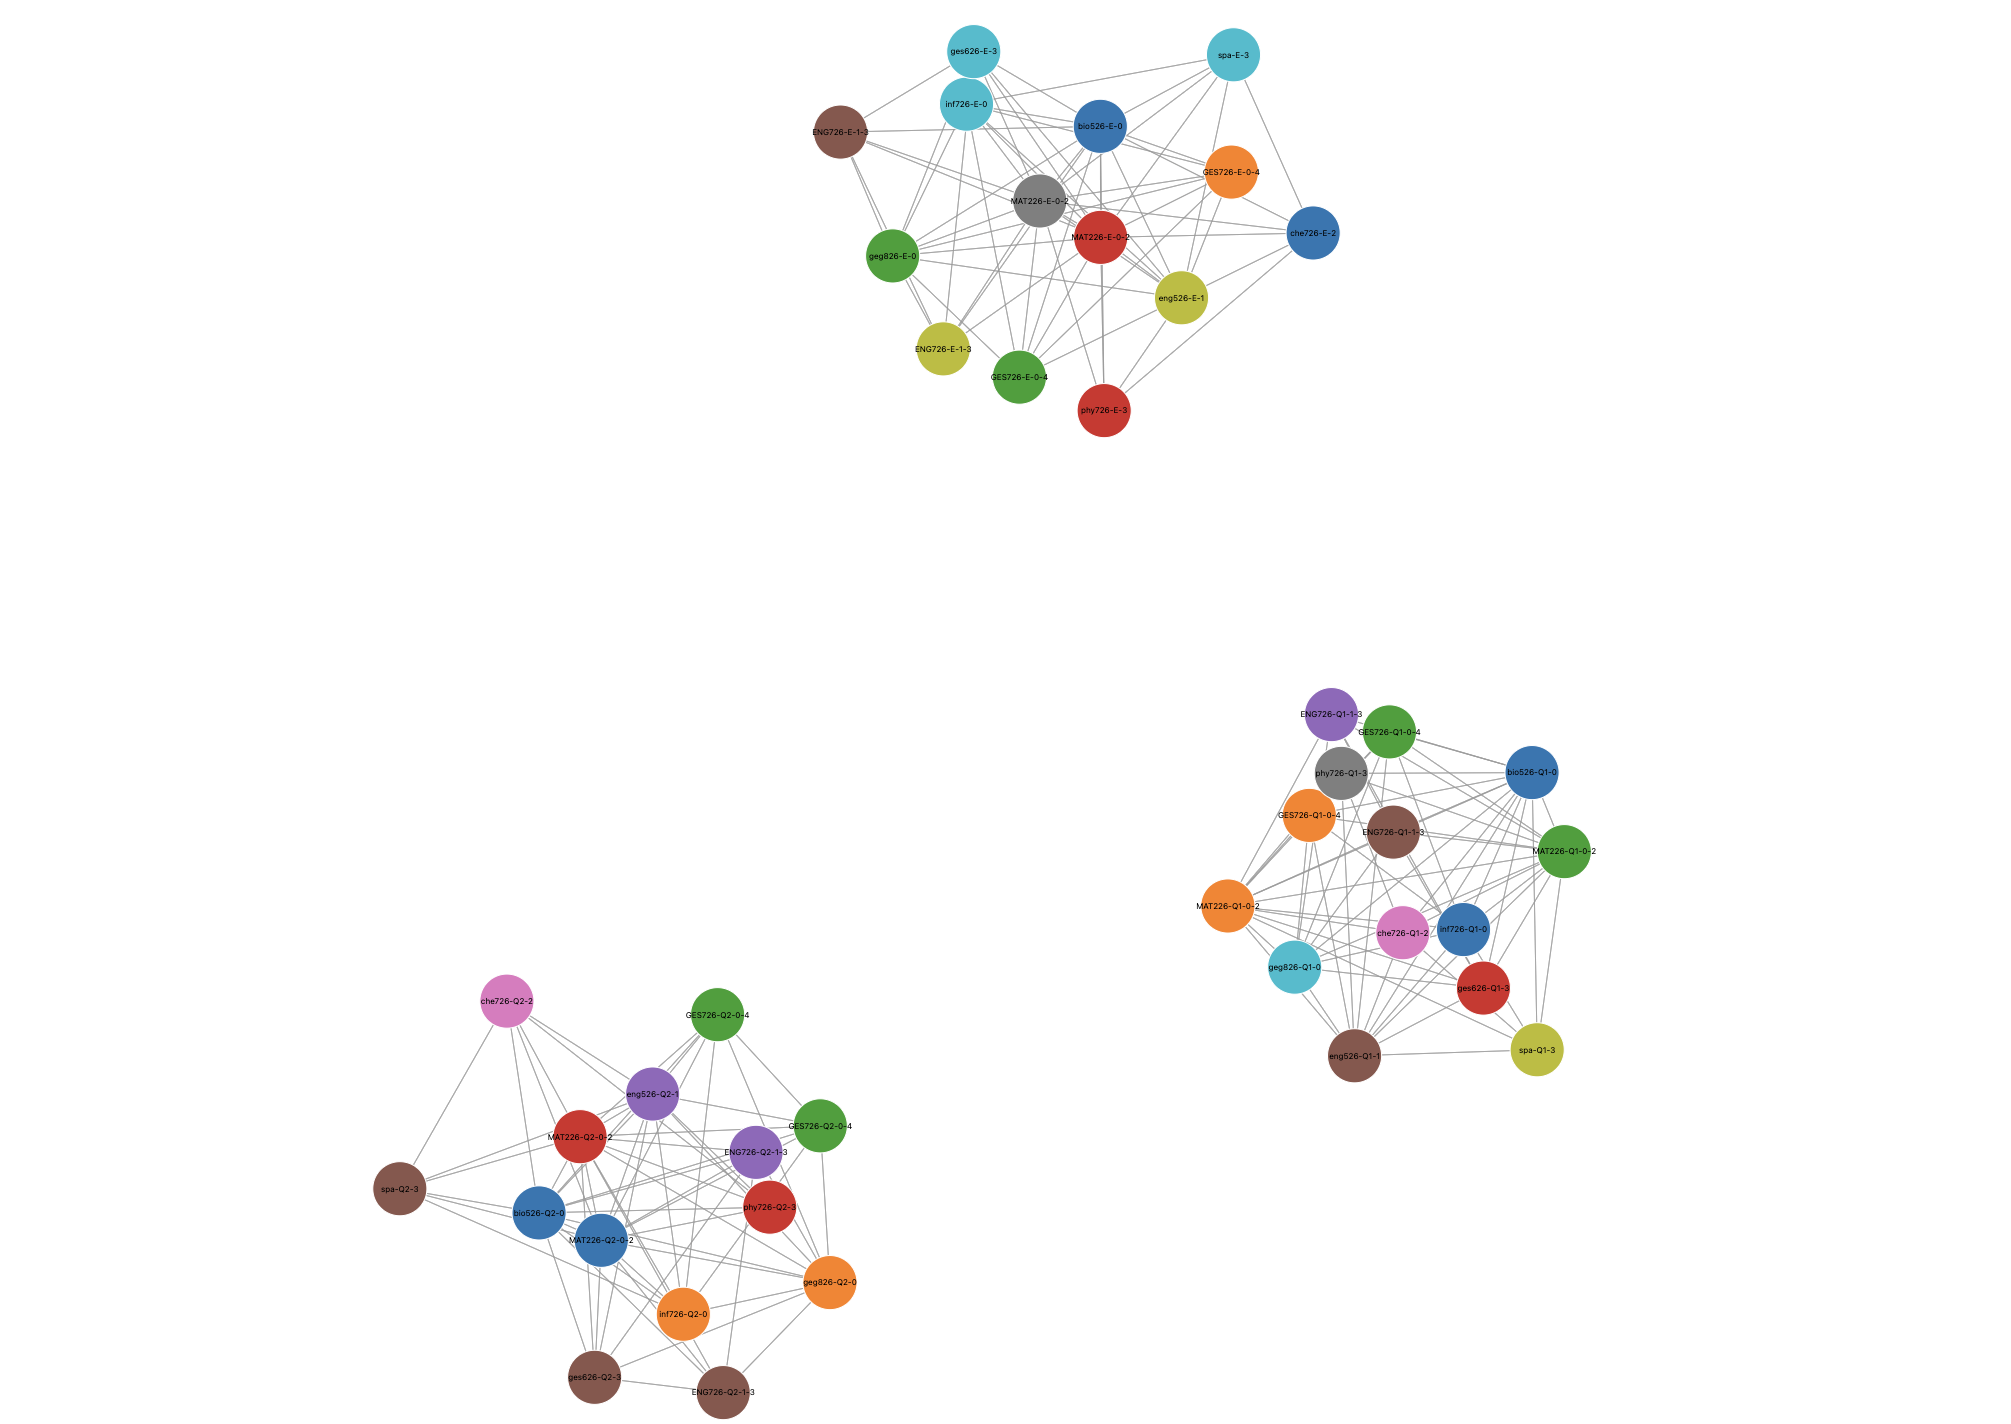
\includegraphics[width=0.5\linewidth]{docs/graphics/graph-all.png}
    \caption{Graph einer beispielhaften Implementierung}
    \label{fig:graph1}
\end{figure}
\begin{figure}[H]
    \centering
    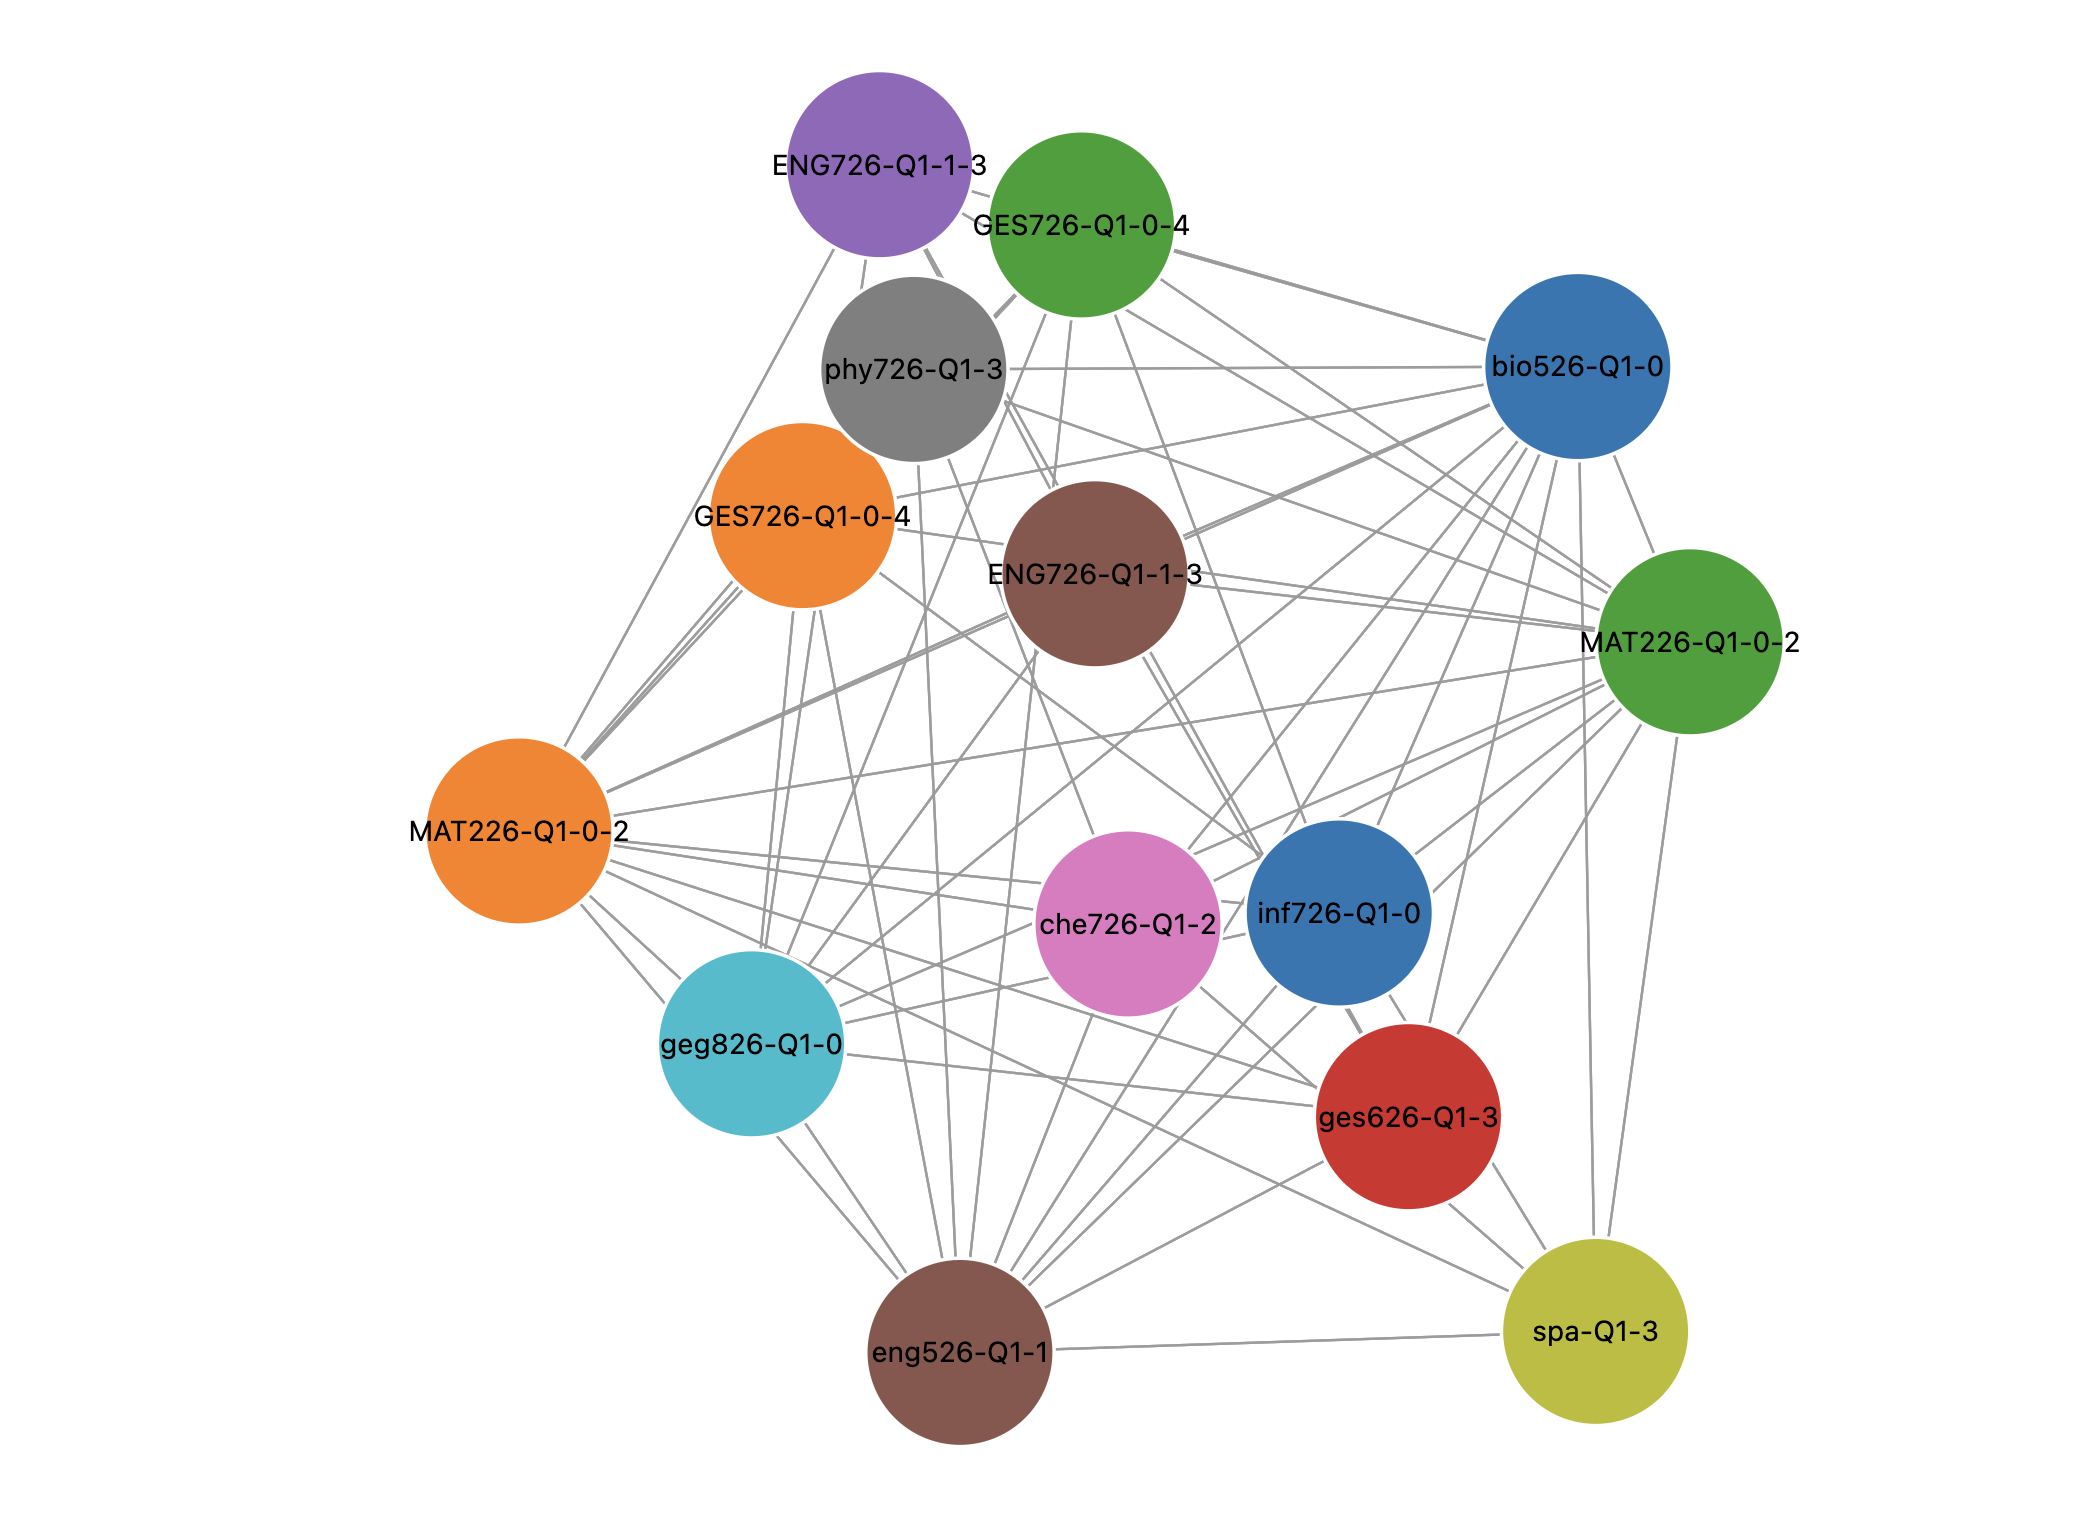
\includegraphics[width=0.5\linewidth]{docs/graphics/graph-detail.png}
    \caption{Teil des Graphen einer beispielhaften Implementierung}
    \label{fig:graph2}
\end{figure}
\begin{figure}[H]
    \centering
    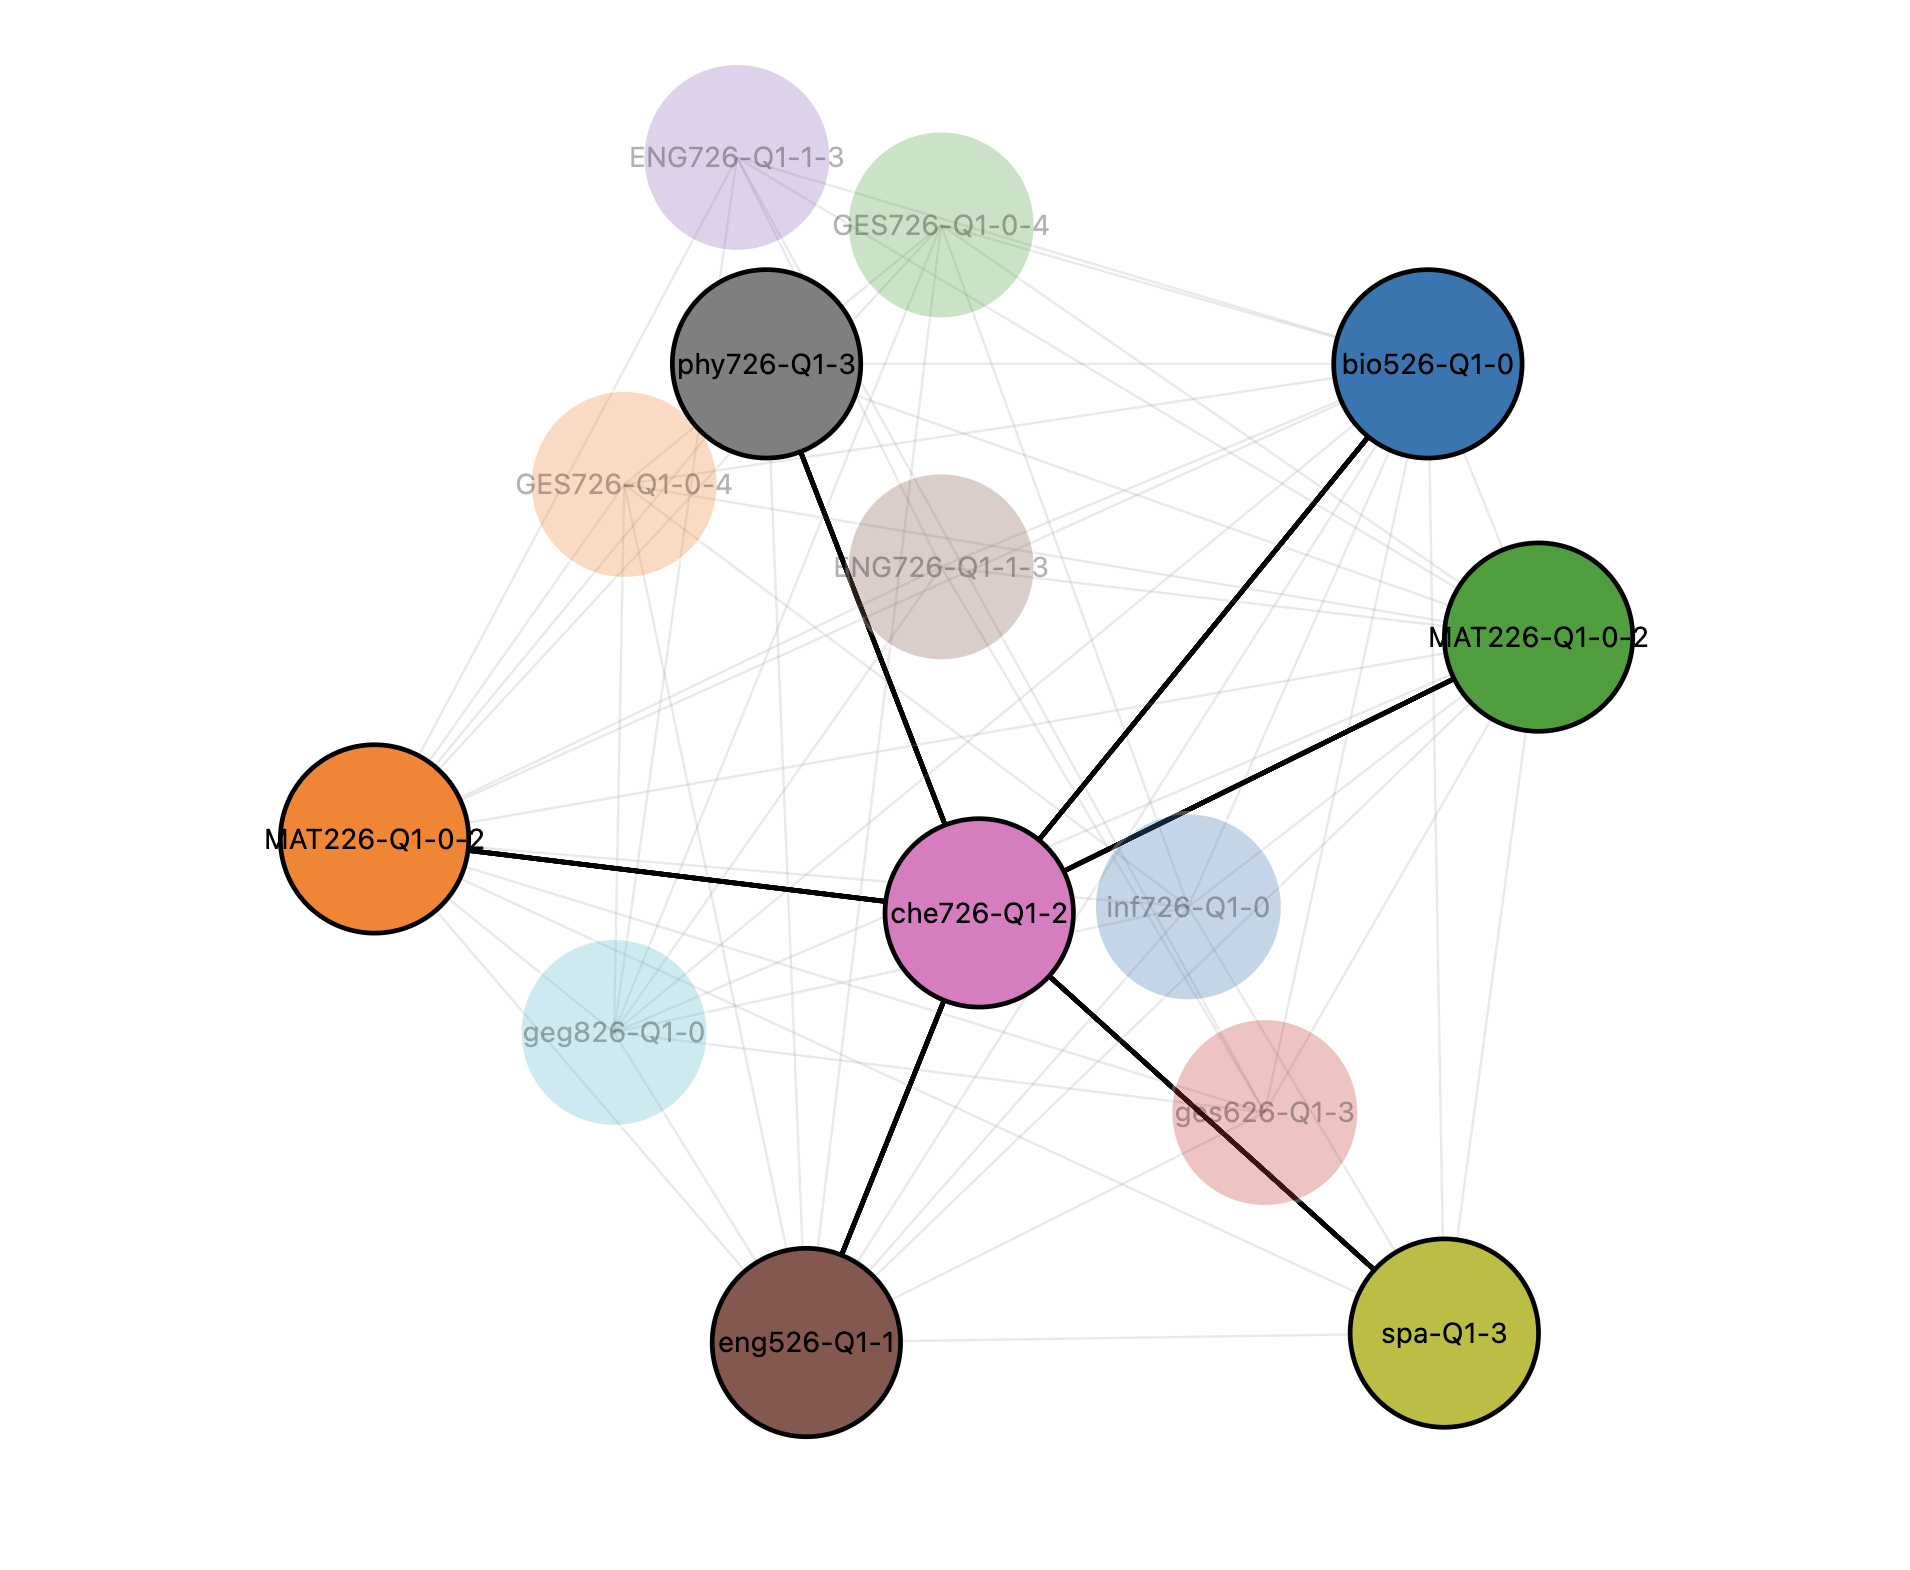
\includegraphics[width=0.5\linewidth]{docs/graphics/graph-detail-selected.png}
    \caption{Teil des Graphen einer beispielhaften Implementierung mit ausgewähltem Knoten}
    \label{fig:graph3}
\end{figure}


\newpage
\subsection{Klausurenplan}
\begin{figure}[H]
    \centering
    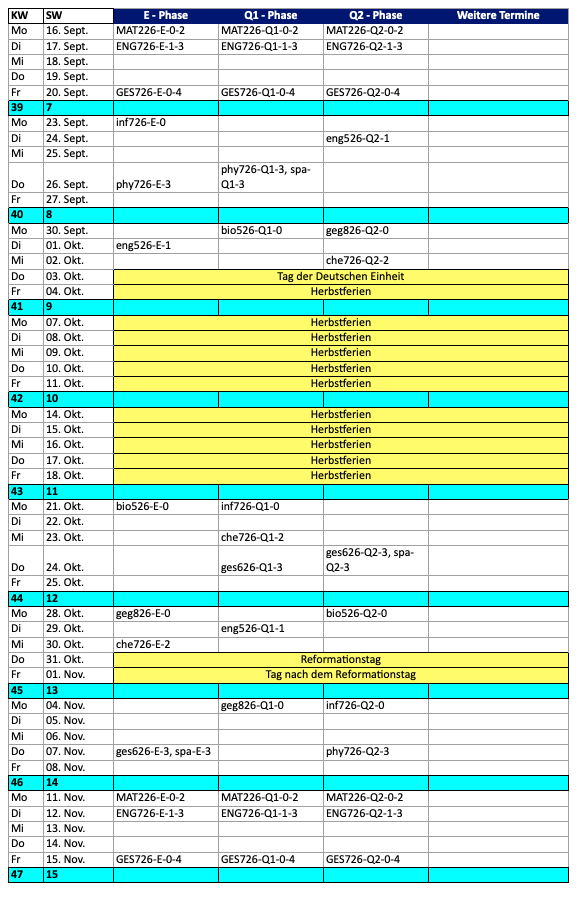
\includegraphics[width=0.8\linewidth]{docs/graphics/Klausurenplan.png}
    \caption{Klausurenplan als Excel-Tabelle}
    \label{fig:klausurenplan}
\end{figure}
Der 16. September ist der Montag, an dem die gewählte Klausurenphase beginnt. Dies ist nicht der Beginn des Schuljahres.
\newpage
\section{Aufteilung der Arbeitsanteile}

\begin{longtable}{|p{3cm}|p{4cm}|p{4cm}|p{4cm}|}
\hline
\textbf{Kapitel Nr.} & \textbf{Kapitel} & \textbf{Tom Kurzke (\%)} & \textbf{Julius Backes (\%)} \\
\hline
\multicolumn{2}{|p{7cm}|}{Entwicklung der Webanwendung (Produkt)} & 0 & 100\\
\hline
1 & Einleitung & 60 & 40 \\
\hline
2 & Grundlagen der Graphentheorie & 35 & 65 \\
\hline
3 & Klausurenplanung als Optimierungsproblem & - & - \\
\hline
4 & Entwicklung der Web-Applikation & 0 & 100 \\
\hline
5 & Mathematische Analyse der Optimierung & - & - \\
\hline
6 & Evaluation und Tests & - & - \\
\hline
7 & Zusammenfassung und Ausblick & - & - \\
\hline
\end{longtable}
\input{docs/chapters/10_erklärung}

\end{document}
